\section{Generaci\'on de c\'odigo ARM}

Para generar c\'odigo ARM se necesita un ensamblador, y un compilador en caso de querer escribir c\'odigo de nivel m\'as alto.

Se evaluaron varias herramientas que existen actualmente, como:

\begin{itemize}
\item CrossWorks
\item MDK-ARM
\item GNU Compiler Collection (GCC)
\end{itemize}

Una de las herramientas m\'as accesibles es la del GCC, es de licencia libre y es la herramienta que se usa por defecto en Linux.

GCC nos provee de las herramientas b\'asicas que deseamos utilizar que son:

\begin{itemize}

\item Ensamblador
\item Compilador de C

\end{itemize}

El \textbf{ensamblador} es el componente que se encarga de convertir el c\'odigo ensamblador en c\'odigo m\'aquina, el ensamblador de GCC lo hace utilizando el formato binario ELF, el cual especifica en qu\'e direcci\'on de memoria se localiza da seccion y donde debe de estar cuando se inicie la ejecuci\'on. El objetivo de este formato binario es el de generar binarios m\'as peque\~nos que indiquen al sistema operativo como se debe de crear el proceso en memoria para su ejecuci\'on.

El \textbf{Compilador} ejecuta una serie de tareas que tienen como objetivo convertir el c\'odigo C en ensamblador para posteriormente utilizar al ensamblador para generar el binario, por ello tambi\'en generar\'a programas ELF.

El formato ELF ayuda mucho para disminuir el tama\~no estableciendo mecanismos de bibliotecas din\'amicas y dandole informaci\'on al sistema operativo para crear la imagen del proceso en ejecuci\'on. Sin embargo nosotros no disponemos de un sistema operativo, por lo que se ha desarrollado una herramienta que genera la imagen del programa binario antes de cargarla al simulador o tarjeta.

\subsection{elf\_read}

Este programa se encarga de generar un binario a partir de un archivo ELF, poniendo el c\'odigo correspondiente en el lugar adecuado del binario. Para poder hacer esto es necesario conocer la estructura que tienen los archivos ELF. A continuaci\'on se puede observar parte de la estructura de los archivos ELF.\medskip

\lstset{language=C}
\lstinputlisting{./elfstruct.h}

Se pueden observar dos estructuras, una es la estructura del header y la otra es la estructura de las secciones. El valor en la variable e\_shnum del header nos dice cuantas secciones tiene el programa. Solo las secciones que tengan asignado un sh\_addr se deben de pasar al binario.\medskip

\begin{figure}[H]
\centering
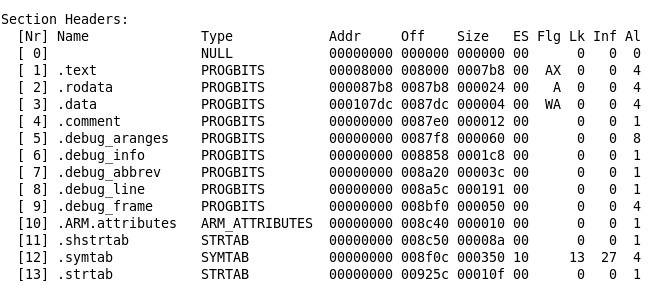
\includegraphics[scale=0.5]{secciones}
\caption{Secciones de un archivo ELF}\label{fig:secciones}
\end{figure}

Por ejemplo en la figura se puede observar que solo las secciones .text, .rodata y .data tiene asignado un Addr por lo tanto solo esas secciones se copiara al binario en esa direcci\'on y se sacara del archivo ELF en la direcci\'on Off conrrespondiente. A continuaci\'on se muestra el binario generado:\medskip

\lstinputlisting{./binario}
